\documentclass[CMPE]{KGCOEReport}
\usepackage{float}
\usepackage{adjustbox}
\graphicspath{ {./images/} }

\newcommand{\name}{Mohammed Fareed \\ Trent Wesley}
\newcommand{\exerciseNumber}{8}
\newcommand{\exerciseDescription}{Heartrate Monitor}
\newcommand{\dateDone}{November 8, 2023}
\newcommand{\dateSubmitted}{November 29, 2023}

\newcommand{\classCode}{CMPE 460}
\newcommand{\LabSectionNum}{1}
\newcommand{\LabInstructor}{Prof.\ Hussin Ketout}
\newcommand{\TAs}{Andrew Tevebaugh \\ Colin Vo}
\newcommand{\LectureSectionNum}{1}
\newcommand{\LectureInstructor}{Prof.\ Hussin Ketout}


\begin{document}
\maketitle

\section*{Abstract}

yeehaw

\section*{Design Methodology}

\begin{figure}[H]
    \centering
    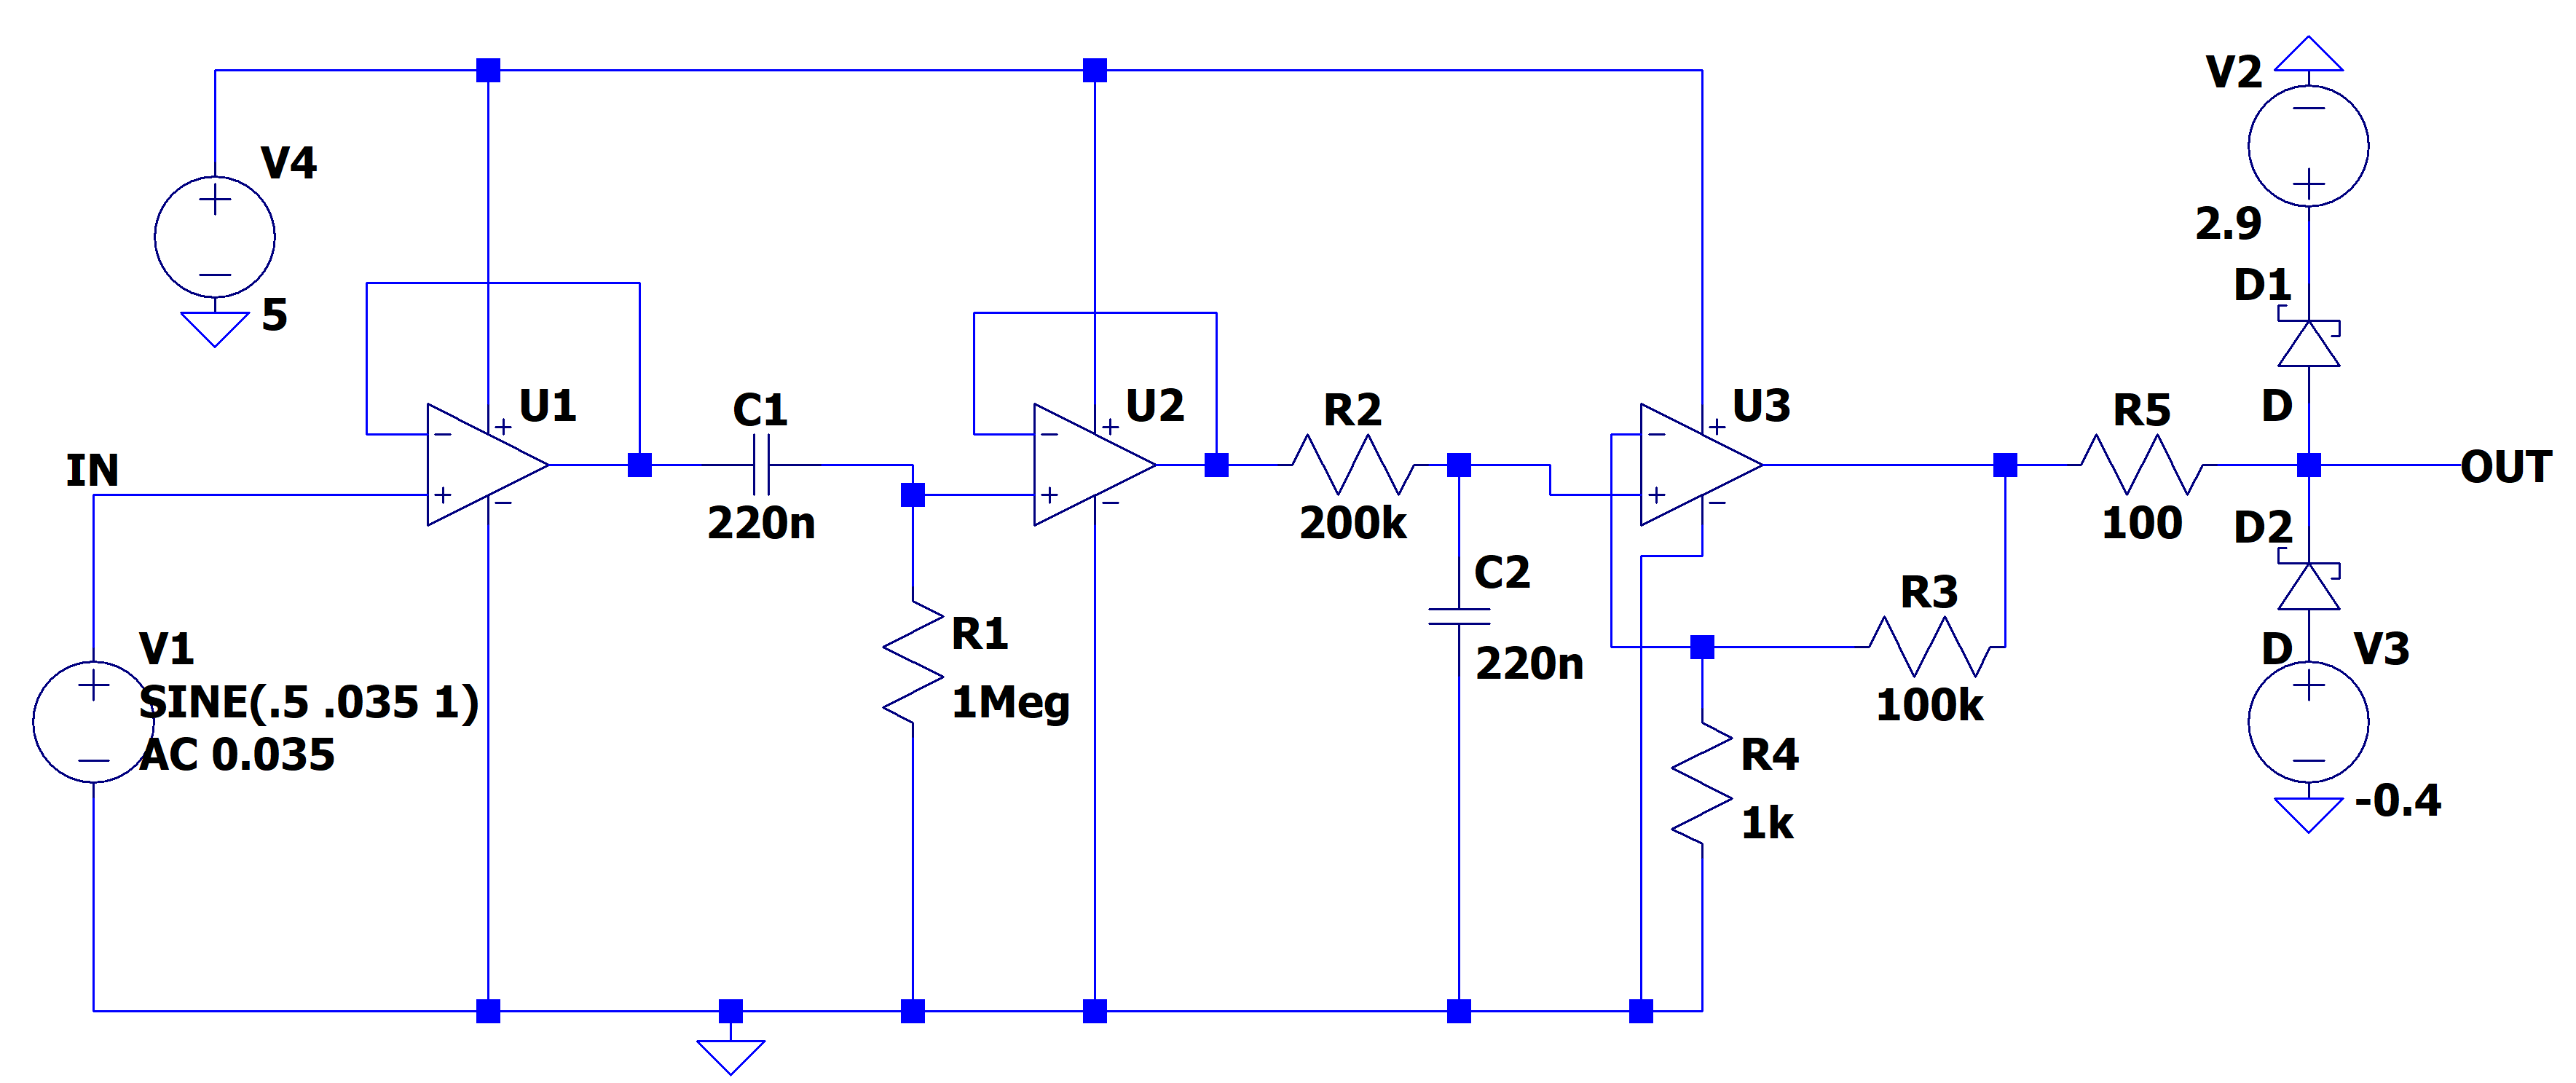
\includegraphics[width=1\textwidth]{LTspiceSchematic.png}
    \caption{LTspice Schematic}
    \label{fig:ltspiceSchematic}
\end{figure}

\section*{Results and Analysis}

\begin{figure}[H]
    \centering
    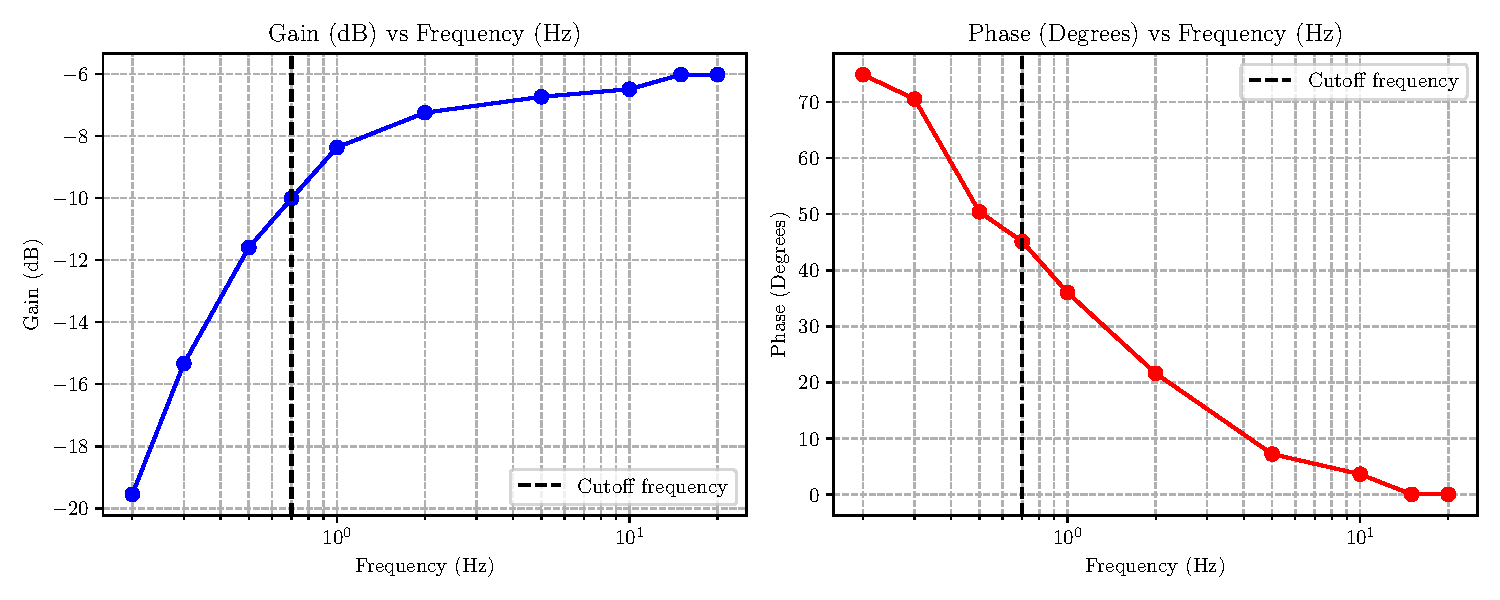
\includegraphics[width=1\textwidth]{high_pass_plot.pdf}
    \caption{High-Pass Filter Bode Plot}
    \label{fig:highPassBode}
\end{figure}

\begin{figure}[H]
    \centering
    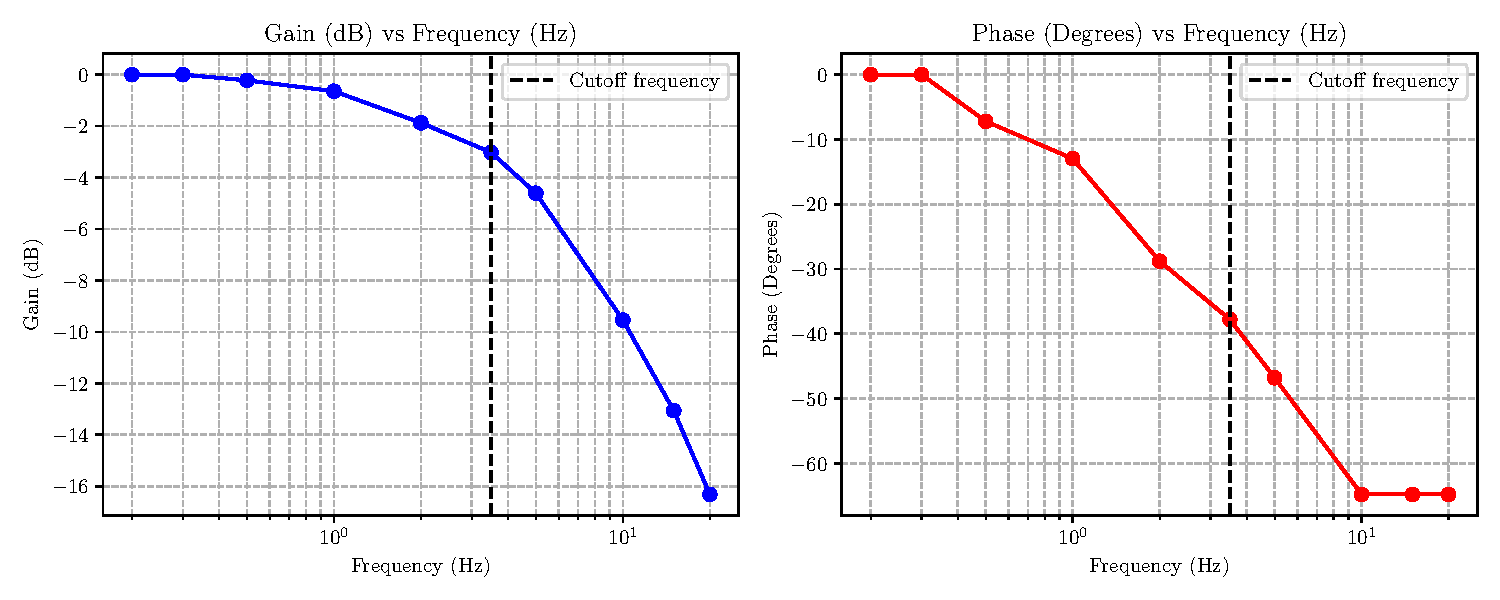
\includegraphics[width=1\textwidth]{low_pass_plot.pdf}
    \caption{Low-Pass Filter Bode Plot}
    \label{fig:lowPassBode}
\end{figure}

\begin{figure}[H]
    \centering
    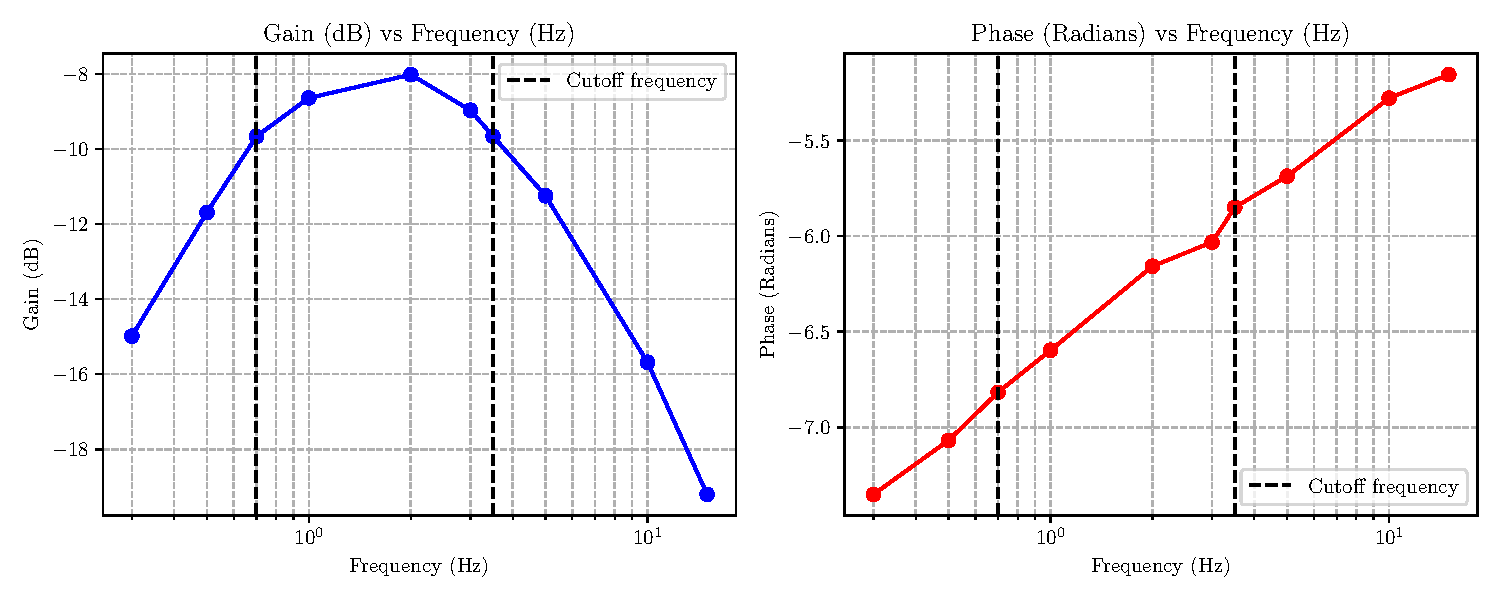
\includegraphics[width=1\textwidth]{band_pass_plot.pdf}
    \caption{Band-Pass Filter Bode Plot}
    \label{fig:bandPassBode}
\end{figure}

\begin{figure}[H]
    \centering
    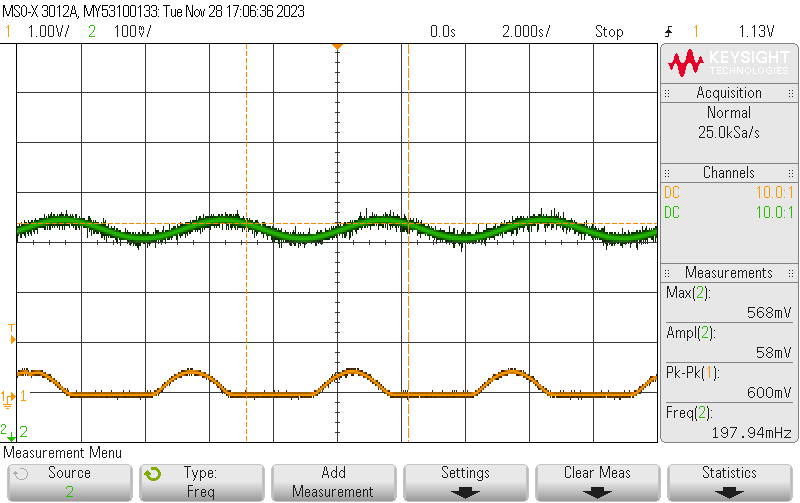
\includegraphics[width=0.75\textwidth]{200mHz.png}
    \caption{Oscilloscope SCHTUFF}
    \label{fig:200mHzCapture}
\end{figure}

\begin{figure}[H]
    \centering
    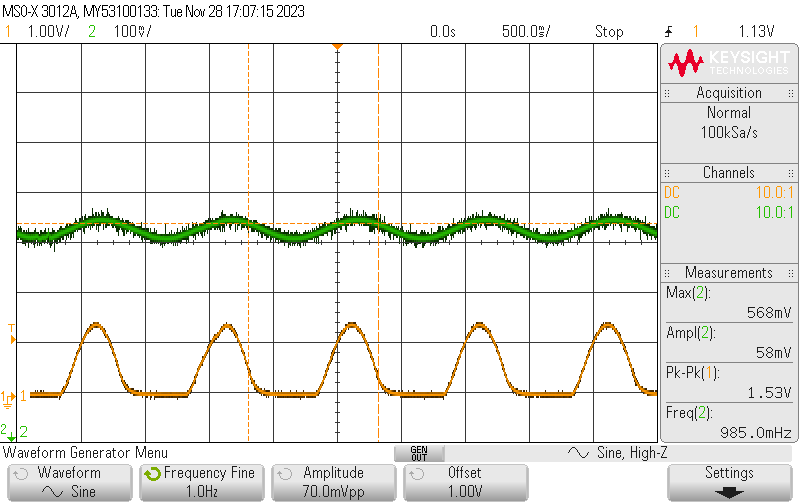
\includegraphics[width=0.75\textwidth]{1Hz.png}
    \caption{Oscilloscope SCHTUFF}
    \label{fig:1HzCapture}
\end{figure}

\begin{figure}[H]
    \centering
    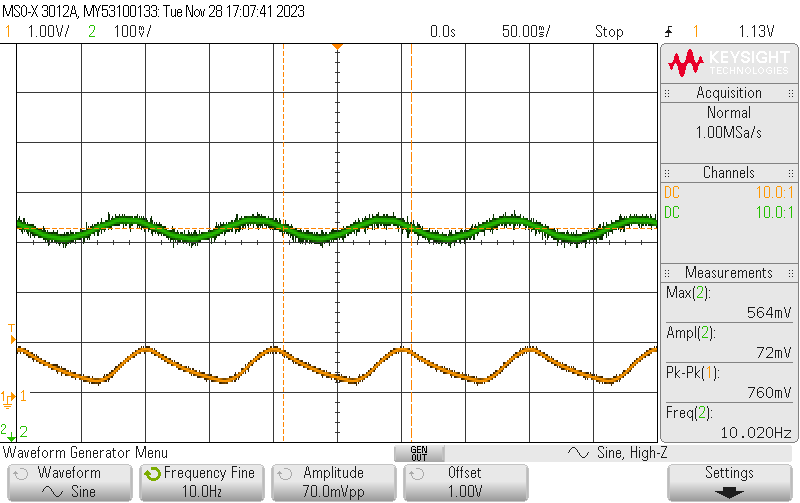
\includegraphics[width=0.75\textwidth]{10Hz.png}
    \caption{Oscilloscope SCHTUFF}
    \label{fig:10HzCapture}
\end{figure}

\section*{Questions}

\textbf{1.} \emph{What is the ERC and DRC for?}

ERC stands for Electrical Rule Check and DRC stands for Design Rule Check. The ERC checks for electrical errors in the schematic, such as unconnected pins. The DRC checks for design errors in the schematic, such as incorrect pin types.

\bigskip

\textbf{2.} \emph{Did your circuit cutoff frequencies match your expected/calculated values? Explain}

\bigskip

\textbf{3.} \emph{Did the gain of the circuit match the expected/calculated values? Explain}

\section*{Conclusion}



\newpage
\begin{figure}[H]
    \centering
    \begin{adjustbox}{center}
        
\includegraphics[width=1.26\textwidth]{signoff.pdf}
    \end{adjustbox}
\end{figure}

\end{document}
